% Created by tikzDevice version 0.12.6 on 2026-10-30 11:47:30
% !TEX encoding = UTF-8 Unicode
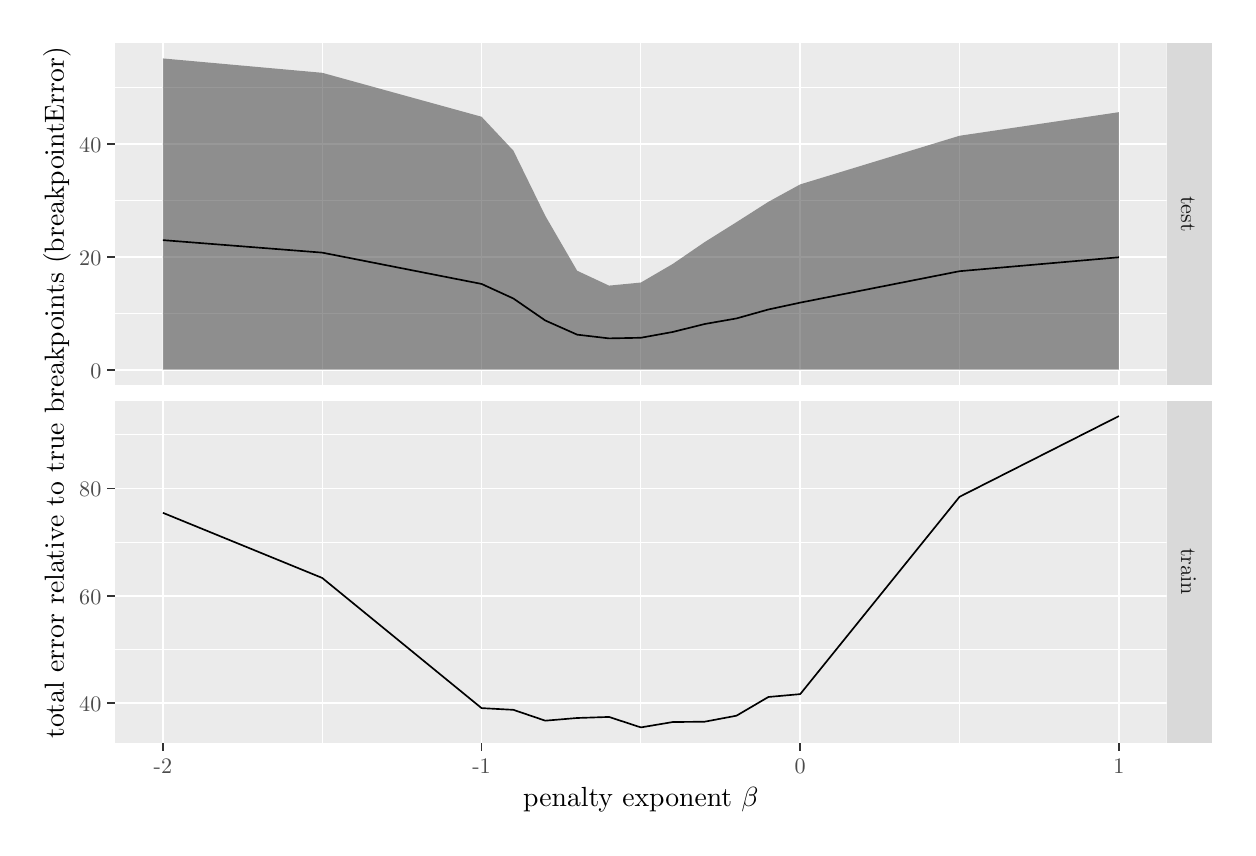
\begin{tikzpicture}[x=1pt,y=1pt]
\definecolor{fillColor}{RGB}{255,255,255}
\path[use as bounding box,fill=fillColor,fill opacity=0.00] (0,0) rectangle (433.62,289.08);
\begin{scope}
\path[clip] (  0.00,  0.00) rectangle (433.62,289.08);
\definecolor{drawColor}{RGB}{255,255,255}
\definecolor{fillColor}{RGB}{255,255,255}

\path[draw=drawColor,line width= 0.6pt,line join=round,line cap=round,fill=fillColor] (  0.00,  0.00) rectangle (433.62,289.08);
\end{scope}
\begin{scope}
\path[clip] ( 31.58,159.84) rectangle (411.58,283.58);
\definecolor{fillColor}{gray}{0.92}

\path[fill=fillColor] ( 31.58,159.84) rectangle (411.58,283.58);
\definecolor{drawColor}{RGB}{255,255,255}

\path[draw=drawColor,line width= 0.3pt,line join=round] ( 31.58,185.86) --
	(411.58,185.86);

\path[draw=drawColor,line width= 0.3pt,line join=round] ( 31.58,226.65) --
	(411.58,226.65);

\path[draw=drawColor,line width= 0.3pt,line join=round] ( 31.58,267.44) --
	(411.58,267.44);

\path[draw=drawColor,line width= 0.3pt,line join=round] (106.43,159.84) --
	(106.43,283.58);

\path[draw=drawColor,line width= 0.3pt,line join=round] (221.58,159.84) --
	(221.58,283.58);

\path[draw=drawColor,line width= 0.3pt,line join=round] (336.73,159.84) --
	(336.73,283.58);

\path[draw=drawColor,line width= 0.6pt,line join=round] ( 31.58,165.47) --
	(411.58,165.47);

\path[draw=drawColor,line width= 0.6pt,line join=round] ( 31.58,206.26) --
	(411.58,206.26);

\path[draw=drawColor,line width= 0.6pt,line join=round] ( 31.58,247.04) --
	(411.58,247.04);

\path[draw=drawColor,line width= 0.6pt,line join=round] ( 48.85,159.84) --
	( 48.85,283.58);

\path[draw=drawColor,line width= 0.6pt,line join=round] (164.01,159.84) --
	(164.01,283.58);

\path[draw=drawColor,line width= 0.6pt,line join=round] (279.16,159.84) --
	(279.16,283.58);

\path[draw=drawColor,line width= 0.6pt,line join=round] (394.31,159.84) --
	(394.31,283.58);
\definecolor{fillColor}{RGB}{51,51,51}

\path[fill=fillColor,fill opacity=0.50] ( 48.85,277.96) --
	(106.43,272.77) --
	(164.01,256.89) --
	(175.52,244.63) --
	(187.04,221.09) --
	(198.55,201.25) --
	(210.07,195.87) --
	(221.58,196.98) --
	(233.10,203.70) --
	(244.61,211.58) --
	(256.13,218.80) --
	(267.64,226.14) --
	(279.16,232.45) --
	(336.73,250.02) --
	(394.31,258.54) --
	(394.31,165.47) --
	(336.73,165.47) --
	(279.16,165.47) --
	(267.64,165.47) --
	(256.13,165.47) --
	(244.61,165.47) --
	(233.10,165.47) --
	(221.58,165.47) --
	(210.07,165.47) --
	(198.55,165.47) --
	(187.04,165.47) --
	(175.52,165.47) --
	(164.01,165.47) --
	(106.43,165.47) --
	( 48.85,165.47) --
	cycle;

\path[] ( 48.85,277.96) --
	(106.43,272.77) --
	(164.01,256.89) --
	(175.52,244.63) --
	(187.04,221.09) --
	(198.55,201.25) --
	(210.07,195.87) --
	(221.58,196.98) --
	(233.10,203.70) --
	(244.61,211.58) --
	(256.13,218.80) --
	(267.64,226.14) --
	(279.16,232.45) --
	(336.73,250.02) --
	(394.31,258.54);

\path[] (394.31,165.47) --
	(336.73,165.47) --
	(279.16,165.47) --
	(267.64,165.47) --
	(256.13,165.47) --
	(244.61,165.47) --
	(233.10,165.47) --
	(221.58,165.47) --
	(210.07,165.47) --
	(198.55,165.47) --
	(187.04,165.47) --
	(175.52,165.47) --
	(164.01,165.47) --
	(106.43,165.47) --
	( 48.85,165.47);
\definecolor{drawColor}{RGB}{0,0,0}

\path[draw=drawColor,line width= 0.6pt,line join=round] ( 48.85,212.31) --
	(106.43,207.79) --
	(164.01,196.48) --
	(175.52,191.21) --
	(187.04,183.27) --
	(198.55,178.15) --
	(210.07,176.80) --
	(221.58,177.03) --
	(233.10,179.12) --
	(244.61,181.99) --
	(256.13,184.01) --
	(267.64,187.24) --
	(279.16,189.72) --
	(336.73,201.08) --
	(394.31,206.11);
\end{scope}
\begin{scope}
\path[clip] ( 31.58, 30.61) rectangle (411.58,154.34);
\definecolor{fillColor}{gray}{0.92}

\path[fill=fillColor] ( 31.58, 30.61) rectangle (411.58,154.34);
\definecolor{drawColor}{RGB}{255,255,255}

\path[draw=drawColor,line width= 0.3pt,line join=round] ( 31.58, 64.35) --
	(411.58, 64.35);

\path[draw=drawColor,line width= 0.3pt,line join=round] ( 31.58,103.17) --
	(411.58,103.17);

\path[draw=drawColor,line width= 0.3pt,line join=round] ( 31.58,141.99) --
	(411.58,141.99);

\path[draw=drawColor,line width= 0.3pt,line join=round] (106.43, 30.61) --
	(106.43,154.34);

\path[draw=drawColor,line width= 0.3pt,line join=round] (221.58, 30.61) --
	(221.58,154.34);

\path[draw=drawColor,line width= 0.3pt,line join=round] (336.73, 30.61) --
	(336.73,154.34);

\path[draw=drawColor,line width= 0.6pt,line join=round] ( 31.58, 44.94) --
	(411.58, 44.94);

\path[draw=drawColor,line width= 0.6pt,line join=round] ( 31.58, 83.76) --
	(411.58, 83.76);

\path[draw=drawColor,line width= 0.6pt,line join=round] ( 31.58,122.58) --
	(411.58,122.58);

\path[draw=drawColor,line width= 0.6pt,line join=round] ( 48.85, 30.61) --
	( 48.85,154.34);

\path[draw=drawColor,line width= 0.6pt,line join=round] (164.01, 30.61) --
	(164.01,154.34);

\path[draw=drawColor,line width= 0.6pt,line join=round] (279.16, 30.61) --
	(279.16,154.34);

\path[draw=drawColor,line width= 0.6pt,line join=round] (394.31, 30.61) --
	(394.31,154.34);
\definecolor{drawColor}{RGB}{0,0,0}

\path[draw=drawColor,line width= 0.6pt,line join=round] ( 48.85,113.78) --
	(106.43, 90.24) --
	(164.01, 43.20) --
	(175.52, 42.58) --
	(187.04, 38.66) --
	(198.55, 39.63) --
	(210.07, 40.01) --
	(221.58, 36.23) --
	(233.10, 38.17) --
	(244.61, 38.29) --
	(256.13, 40.46) --
	(267.64, 47.22) --
	(279.16, 48.26) --
	(336.73,119.56) --
	(394.31,148.72);
\end{scope}
\begin{scope}
\path[clip] (411.58,159.84) rectangle (428.12,283.58);
\definecolor{fillColor}{gray}{0.85}

\path[fill=fillColor] (411.58,159.84) rectangle (428.12,283.58);
\definecolor{drawColor}{gray}{0.10}

\node[text=drawColor,rotate=-90.00,anchor=base,inner sep=0pt, outer sep=0pt, scale=  0.80] at (416.84,221.71) {test};
\end{scope}
\begin{scope}
\path[clip] (411.58, 30.61) rectangle (428.12,154.34);
\definecolor{fillColor}{gray}{0.85}

\path[fill=fillColor] (411.58, 30.61) rectangle (428.12,154.34);
\definecolor{drawColor}{gray}{0.10}

\node[text=drawColor,rotate=-90.00,anchor=base,inner sep=0pt, outer sep=0pt, scale=  0.80] at (416.84, 92.47) {train};
\end{scope}
\begin{scope}
\path[clip] (  0.00,  0.00) rectangle (433.62,289.08);
\definecolor{drawColor}{gray}{0.20}

\path[draw=drawColor,line width= 0.6pt,line join=round] ( 48.85, 27.86) --
	( 48.85, 30.61);

\path[draw=drawColor,line width= 0.6pt,line join=round] (164.01, 27.86) --
	(164.01, 30.61);

\path[draw=drawColor,line width= 0.6pt,line join=round] (279.16, 27.86) --
	(279.16, 30.61);

\path[draw=drawColor,line width= 0.6pt,line join=round] (394.31, 27.86) --
	(394.31, 30.61);
\end{scope}
\begin{scope}
\path[clip] (  0.00,  0.00) rectangle (433.62,289.08);
\definecolor{drawColor}{gray}{0.30}

\node[text=drawColor,anchor=base,inner sep=0pt, outer sep=0pt, scale=  0.80] at ( 48.85, 19.62) {-2};

\node[text=drawColor,anchor=base,inner sep=0pt, outer sep=0pt, scale=  0.80] at (164.01, 19.62) {-1};

\node[text=drawColor,anchor=base,inner sep=0pt, outer sep=0pt, scale=  0.80] at (279.16, 19.62) {0};

\node[text=drawColor,anchor=base,inner sep=0pt, outer sep=0pt, scale=  0.80] at (394.31, 19.62) {1};
\end{scope}
\begin{scope}
\path[clip] (  0.00,  0.00) rectangle (433.62,289.08);
\definecolor{drawColor}{gray}{0.30}

\node[text=drawColor,anchor=base east,inner sep=0pt, outer sep=0pt, scale=  0.80] at ( 26.63,162.45) {0};

\node[text=drawColor,anchor=base east,inner sep=0pt, outer sep=0pt, scale=  0.80] at ( 26.63,203.24) {20};

\node[text=drawColor,anchor=base east,inner sep=0pt, outer sep=0pt, scale=  0.80] at ( 26.63,244.03) {40};
\end{scope}
\begin{scope}
\path[clip] (  0.00,  0.00) rectangle (433.62,289.08);
\definecolor{drawColor}{gray}{0.20}

\path[draw=drawColor,line width= 0.6pt,line join=round] ( 28.83,165.47) --
	( 31.58,165.47);

\path[draw=drawColor,line width= 0.6pt,line join=round] ( 28.83,206.26) --
	( 31.58,206.26);

\path[draw=drawColor,line width= 0.6pt,line join=round] ( 28.83,247.04) --
	( 31.58,247.04);
\end{scope}
\begin{scope}
\path[clip] (  0.00,  0.00) rectangle (433.62,289.08);
\definecolor{drawColor}{gray}{0.30}

\node[text=drawColor,anchor=base east,inner sep=0pt, outer sep=0pt, scale=  0.80] at ( 26.63, 41.92) {40};

\node[text=drawColor,anchor=base east,inner sep=0pt, outer sep=0pt, scale=  0.80] at ( 26.63, 80.74) {60};

\node[text=drawColor,anchor=base east,inner sep=0pt, outer sep=0pt, scale=  0.80] at ( 26.63,119.56) {80};
\end{scope}
\begin{scope}
\path[clip] (  0.00,  0.00) rectangle (433.62,289.08);
\definecolor{drawColor}{gray}{0.20}

\path[draw=drawColor,line width= 0.6pt,line join=round] ( 28.83, 44.94) --
	( 31.58, 44.94);

\path[draw=drawColor,line width= 0.6pt,line join=round] ( 28.83, 83.76) --
	( 31.58, 83.76);

\path[draw=drawColor,line width= 0.6pt,line join=round] ( 28.83,122.58) --
	( 31.58,122.58);
\end{scope}
\begin{scope}
\path[clip] (  0.00,  0.00) rectangle (433.62,289.08);
\definecolor{drawColor}{RGB}{0,0,0}

\node[text=drawColor,anchor=base,inner sep=0pt, outer sep=0pt, scale=  1.00] at (221.58,  7.63) {penalty exponent $\beta$};
\end{scope}
\begin{scope}
\path[clip] (  0.00,  0.00) rectangle (433.62,289.08);
\definecolor{drawColor}{RGB}{0,0,0}

\node[text=drawColor,rotate= 90.00,anchor=base,inner sep=0pt, outer sep=0pt, scale=  1.00] at ( 13.04,157.09) {total error relative to true breakpoints (breakpointError)};
\end{scope}
\end{tikzpicture}
